\sloppy

\section{Thesis Overview}

The aim of this Thesis was to use observations at far-IR and sub-mm wavelengths, predominantly from the \textit{Herschel Space Observatory}, to investigate the dust properties of active star forming galaxies, to understand the role that they play in the galaxy building epoch of the Universe and to study the evolution of the dust content of galaxies across time. We recall the research questions underpinning the research in this Thesis, that were presented in Chapter \ref{chapter:Introduction}: How has the dust content of galaxies evolved to the present day? Are the dust properties of galaxies the same at all cosmic epochs? And in what evolutionary stage do we observe dust-enshrouded, IR-bright galaxies; do they provide the link to the massive systems we observe in the local Universe today? 

This work heavily relies on \textit{Herschel} selected samples in order to make progress answering these questions. Starting with the H-ATLAS project, for which we present a comprehensive data release of near-IR counterparts in the SGP, and then use to derive their dust masses and the evolution in the space density of dust over the past $8\,$Gyr. We also make use of HerBS and the SPT-SZ survey, which represents a collection of some of the brightest IR galaxies known, allowing us to investigate their dust properties and determine if they are comparable to the local Universe. This is of particular importance to extragalactic studies at high redshifts where it is not uncommon to assume that the dust is non-evolving and is therefore the same as Galactic and local galaxy interstellar dust. Finally, we make use of the HerMES coverage of COSMOS to utilize the exceptional multiwavelength coverage in the field and gain insight into the evolutionary stage of high redshift \textit{Herschel} galaxies.

Below we outline the key results obtained from this Thesis and present possible areas of research that would expand on this work.

\section{Key Results}

In Chapter \ref{chapter:Data_Release_3}, we presented the third data release of the \textit{Herschel}-ATLAS, where we used the well-established Likelihood Ratio method to identify near-IR counterparts from the VISTA VIKING survey.

\begin{itemize}
    \item We estimated that the fraction of \textit{Herschel} detected galaxies that have an associated counterpart on the near-IR images is approximately $83\%$. From a total of $193,527$ sources in the South Galactic Pole field, $110,374$ ($57\%$) were reliably matched to a VIKING galaxy with a probability of being the true identification $> 80\%$. The probability of such an association was calculated using the ratio between the likelihood of the true counterpart being found in the vicinity of the \textit{Herschel} source, and the likelihood of a background interloper being found in the same location with the same $K_s$-band magnitude.
    \item The expected false identification rate of our Bayesian analysis, that is the percentage of \textit{Herschel} sources where we might expect to have matched erroneously with a VIKING counterpart, was approximately $5\%$. Despite this, the completeness of our SGP sample was $78\%$, which represents the fraction of \textit{Herschel} sources where we have secure far-IR and near-IR detections that we were able to recover.
    \item We searched for gravitational lensing events in the SGP field. The most efficient way to select strong lensing events is to target the brightest sources since the number counts of unlensed sources falls rapidly beyond $\sim100\,$mJy at $500\,\mu$m (e.g. \citealt{Vieira_2010, Wardlow_2013, Nayyeri_2016, Negrello_2017}). We presented $41$ bright candidates in the SGP, $11$ of which had not previously been catalogued as strongly lensed galaxies (SLGs), suggesting that the surface density of SLGs is $\sim0.14\,$deg$^{-2}$. Following this, we suggested a new method for predicting the number of lensing events in a blank field using the photometric redshifts of the \textit{Herschel} source and their optical/IR counterparts. We estimated that $\sim6,000$ lensing events might be present in the $\sim300\,$deg$^{2}$ field. This is higher than predicted by galaxy evolution models (e.g. \citealt{Negrello_2007, Cai_2013}), which we attribute to the inclusion of weak gravitational lensing events, not currently accounted for in models.
\end{itemize}

In Chapter \ref{chapter:Dust_Mass_Functions}, we derived dust masses for the galaxies in the SGP and derived the dust mass function in redshift slices of width $0.2$ out to $z = 1$.

\begin{itemize}
    \item To estimate the dust masses of our sample, we first fitted modified blackbody models to their far-IR spectra to derive the luminosity weighted temperatures of the dust. We found that the median dust temperature is $\sim20\,$K and remains roughly constant from $z = 0$ to $z = 1$.
    \item We derived binned dust mass functions in two ways: first by assuming that all galaxies can be described by a single SED with a dust temperature of $20\,$K (in order to assume a uniform luminosity limit across the sample), and second, by allowing the dust temperature to be a free parameter in the SED fitting between $15$ and $25\,$K. The two DMFs were in reasonable agreement at all redshifts. We estimated that the galaxies detected by \textit{Herschel} were typically between $25$ and $60$ times dustier at $z = 1$ than they are locally, dependent on the distribution of dust temperatures.
    \item The integration of our DMFs at each redshift interval gave us measurements for the total amount of dust in galaxies at different epochs, from which we could estimate the dust mass density evolution from $8\,$Gyr in the past to the present day. In agreement with previous H-ATLAS studies that have measured the dust mass density out to $z\sim0.5$ (e.g. \citealt{Dunne_2011}), we observed a rapid decrease in dust density to $z = 0$, by a factor of approximately $2$. The decrease in dust density over the last $8$ billion years can be attributed to a depletion of dust due to star formation, dust destruction outweighing production, or dust lost from the galaxy to its halo.
    \item There is tentative evidence of a peak in the dust mass density at $z\sim0.8 - 1$, although this is subject to potentially large uncertainties in the highest redshift bin. When compared to measurements of the star formation rate density collated in the literature, which show a definitive peak at $z\sim2$, we predict a short timescale of approximately $2$ to $3\,$Gyr between the peak in the star formation rate density and dust mass density. This would suggest that dust production pathways from stellar sources likely form a substantial amount of dust.
\end{itemize}

In Chapter \ref{chapter:Dust_Evolution}, we studied the dust properties of a sample of $\sim 100$ galaxies between $z = 2$ and $z = 6$. We are particularly interested in their measured values of the dust emissivity index, $\beta$, an observational indicator of the physical and chemical properties of the dust grains.

\begin{itemize}
    \item We modelled the IR to mm spectra of these galaxies using three variants of an isothermal modified blackbody model. One assuming optically thin dust, one assuming a general opacity law where the transition between optically thin and optically thick dust occurs at $100\,\mu$m, and the other at $200\,\mu$m. We found that the general opacity models systematically measure lower dust masses and higher dust temperatures than the optically thin model. The dust emissivity index and IR luminosities, however, are insensitive to the chosen model.
    \item We observed a strong relationship between the dust emissivity index and the dust temperature of galaxies, a reflection of the well-known $\beta$-dust temperature degeneracy. We test whether this relationship is an intrinsic property of galaxies or an artefact of the fitting process by running simulations of mock galaxies and attempting to recover the anti-correlation. The correlation between the two parameters for mock galaxies was not strong enough to account for the relationship observed for real galaxies, suggesting that there is a genuine inverse correlation.
    \item The average dust emissivity spectral index was $\beta = 1.96$ ($1.98$ and $1.91$ for SPT and HerBS galaxies, respectively). This value is significantly higher than the value in the Galaxy which is uniformly around $1.51$, and higher than nearby galaxies (\citealt{Lamperti_2019}), suggesting that studies of extragalactic sources at high redshift should favour $\beta \sim 2$ rather than assuming a local value. Within the population studied here, no redshift evolution is observed between $z = 2$ and $z = 6$.
    \item Given the strong relationship between IR luminosity and dust temperature, we selected a sub-sample of galaxies at similar luminosities and found that there appears little evolution in their dust temperatures with redshift.
\end{itemize}

In Chapter \ref{chapter:Radio_Identifications}, we made use of the correlation between far-IR and radio emission of star forming galaxies to identify $3\,$GHz counterparts to \textit{Herschel} sources in COSMOS. With the high angular resolution of our radio IDs, we unambiguously identified multiwavelength counterparts spanning the UV to IR spectrum, from which we studied the evolutionary state of \textit{Herschel} galaxies.

\begin{itemize}
    \item We identified secure radio associations for $1,053$ sources with $250\,\mu$m flux densities $>30\,$mJy. Approximately $15\%$ of these sources had more than one identification. When multiple components were ordered by their radio flux contribution, the brightest counterpart contributed $\sim70\%$ of the integrated radio flux on average, suggesting that the dust emission may emanate from more than one dusty galaxy that are blended together within the \textit{Herschel} beam. These multiple associations often have photometric redshifts in good agreement with each other, suggesting that these real sources may be part of a group or cluster of galaxies. Moreover, at the average redshift of our sample, the separation between radio IDs is between $10$ and $100\,$kpc, which further advocates for clusters of galaxies, confused within a single \textit{Herschel} beam.
    \item The IR spectrum of each galaxy was used to estimate their star formation rates, and the UV-IR coverage from the COSMOS2020 catalogue to estimate their stellar masses. In the SFR-stellar mass plane we observed that our \textit{Herschel} galaxies lie significantly above the star formation main sequence, in a "starbursting" phase with high stellar masses. The time it would take for these galaxies to form their stellar mass is on average $10\%$ of the age of the Universe at which we observe them, suggesting that they have very short starburst lifetimes. The fact that they produce a vast quantity of their stellar mass during a bursting phase suggests they may subsequently evolve rapidly to being passive galaxies with stars of similar ages - an indication that they may be the progenitors of the massive ellipticals observed locally.
    \item We presented a proof-of-concept study for a new method that uses all the properties of the possible counterparts, from the UV to IR photometry, not just the flux density in a single band as is implemented in the LR method, to estimate the probability of association with the far-IR source. We conclude that a Machine Learning algorithm that uses all available bands, as well as the radial offset from the source, would have greater success at correctly identifying our counterparts than current methods.
\end{itemize}

\section{Future Work}

During this Thesis, we have presented four\footnote{On the basis that each chapter corresponds approximately to its own study.} studies that broadly fall under two general topics: i) investigations into the methods used to identify DSFGs and their multiwavelength counterparts, and ii) the use of the full stellar and dust emitting spectra of star forming galaxies to understand the formation and evolution of bright, far-IR detected galaxies. In brief, we have applied statistical techniques to identify near-IR counterparts to \textit{Herschel} sources in H-ATLAS and radio IDs (from which we could utilize the extensive COSMOS coverage) to sources in HerMES (topic i). We have then used these samples to investigate how the quantity of dust in the Universe has changed with time, whether the dust appears similar at all times in cosmic history, and what role these sources play in the formation of galaxies at early times (topic ii). As a result of this breadth, there are many research studies that could follow from the work presented here.

\begin{itemize}
\item \textbf{The Southern H-ATLAS Regions $K_s$-band Survey (SHARKS)}

During the course of this work, a deep VISTA survey called the \textit{Southern H-ATLAS Regions $K_s$-band Survey} (SHARKS; \citealt{Dannerbauer_2022}) provided the first data release from $20\,$deg$^2$ across the SGP, GAMA15 and GAMA12 fields. The project was granted $1,200$ hours of observing time to cover $\sim 300\,$deg$^2$ over large swathes of the H-ATLAS, reaching a $5\sigma$ depth of $\sim22.7$ AB mag in the $K_s$ band, compared to $21.2$ by VIKING. One of the principle aims of this survey is to provide the optimal counterpart identifications for $\sim90\%$ of sources between $z=0$ and $z=3$ by H-ATLAS, ASKAP, SKA and LOFAR (\citealt{Dannerbauer_2022}). Figure \ref{fig:SHARKS_depth} shows the $K_s$-band magnitude as a function of redshift for \textit{Herschel} sources in HerMES, illustrating how the completed SHARKS observations will enable the detection of $90\%$ of H-ATLAS sources. The release of this data would allow us to extend the studies presented in this Thesis, for instance, the evolution in the dust mass function could be extended toward $z = 3$, which would place much tighter constraints on the peak in dust density. This would allow us to consider, for the first time, models of dust production and destruction in accordance with the star formation rate density and dust density of the Universe, concurrently.

\begin{figure}
    \centering
	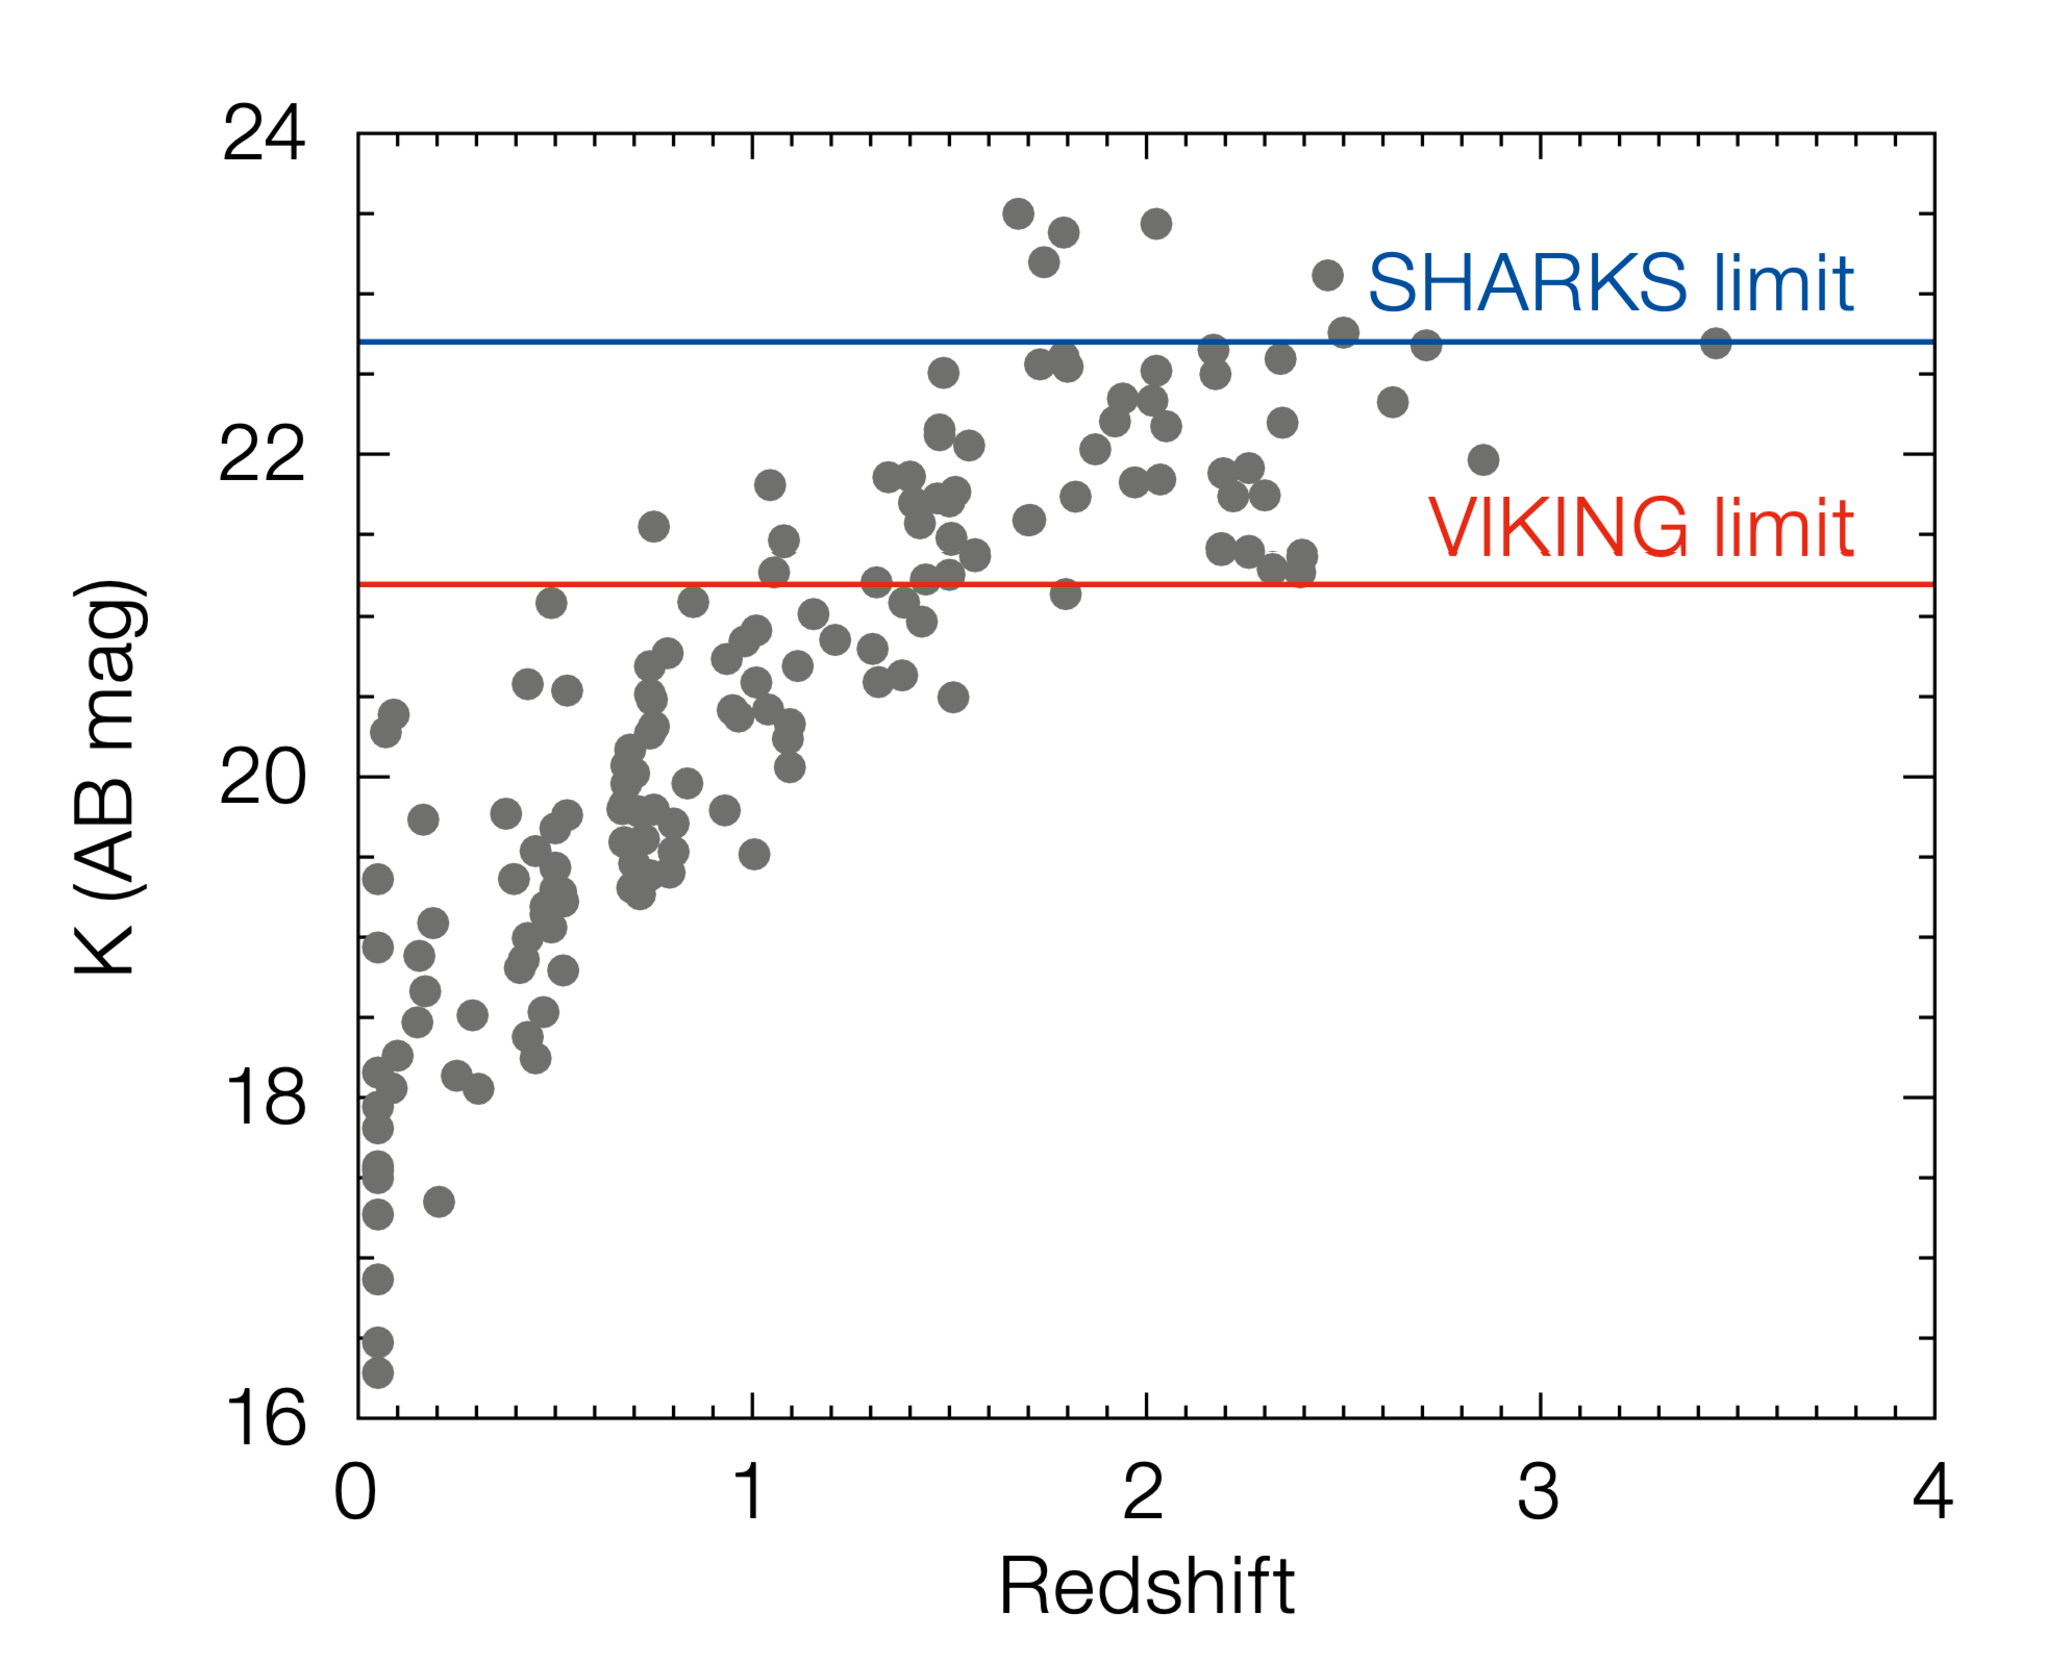
\includegraphics[width=0.75\columnwidth]{Figures/SHAKRS_depth.pdf}
	\caption[$K_s$-band magnitude of HerMES sources as a function of redshift]{The $K_s$-band magnitude of \textit{Herschel} sources in HerMES as a function of redshift, presented in \citealt{Dannerbauer_2022}. The limits of the VIKING and SHARKS surveys are illustrated with red and blue lines, respectively.}
	\label{fig:SHARKS_depth}
\end{figure}

\item \textbf{Machine Learning Algorithm for Counterpart Identification}

At the end of Chapter \ref{chapter:Radio_Identifications} we introduced the idea that current methods for locating counterparts to low resolution sources are limited by the amount of information about the counterpart that is used when assigning probabilities of association. In the two methods used in this Thesis, the Likelihood Ratio method and the frequentist method of \citealt{Lilly_1999}, only the distance from the source and the flux density of a single band is used, requiring us to set lower limits (upper limits in the case of the frequentist method) for the probability that we have identified the true ID, based on arguments of maximizing completeness and minimizing false identifications. We show that DSFG and non-DSFG populations show clear differences in their colours which could be used to improve our confidence in our ID selection. In the first steps of this study, we note that any Machine Learning algorithm that will attempt to select DSFGs from blank fields requires a training set in order to learn the typical properties of these galaxies. We advocate for the sample presented in Chapter \ref{chapter:Radio_Identifications}, as the manner in which the counterparts were selected gives us confidence that we have very few misidentified counterparts (we predict this rate to be $\sim0.5\%$). However, we concede that the sample is not complete with $\sim20\%$ of sources with $250\,\mu$m flux densities $>30\,$mJy missing, and we currently do not have any firm conclusions about what sub-sample of the population these galaxies refer to. As a result, we propose that the first steps in this study, prior to developing a new a binary classification system (DSFG or non-DSFG) that uses the added information from their UV-IR colours, would be to identify if these galaxies represent an underrepresented population of the training set. 

%Secondly, we make it that a Machine Learning algorithm that outputs a binary classification (DSFG or non-DSFG) is not really appropriate, as it provides little context as to the decision making. We can test the performance of the algorithm by using a test set, but we note that this will only be suitable for the sample used here and future surveys would require creating their own training and test sets, which would defeat the purpose of the algorithm. As a result, we would ideally require some metric from which this decision is made that is consistent regardless of the number of photometric bands are available to each source and is thus applicable to future surveys.

\end{itemize}

\section{Concluding Remarks}

With no future plans for a far-IR space telescope to replace \textit{Herschel}, the wide area surveys on which this work is based are not likely to be superseded in the near future. As such, our knowledge about dust in extragalactic sources will likely depend on \textit{Herschel} observations for many more years. This research represents a small addition to the thousands of scientific papers that have utilized \textit{Herschel} observations (likewise SPT) to study how galaxies formed and evolved in the early Universe.
